\section{Technologies}

\subsection{Monitoring Techniques}

\subsubsection{Process Monitor}

One of the most basic forms of monitoring applications is called system monitoring \citep{WhatisaS27:online}, where the target application is monitored using the operating system's process manager which keeps track of resource usages from each of the running processes. This works well for small monolithic applications where there is only one application per server.

\subsubsection{Hypervisor Based Monitor}

Around the time of the early 2000s, a new way of managing servers called virtualisation became popular \citep{Whatisvi12:online}. The idea behind this was to have one big server split into smaller isolated \ac{vm} which made sharing and managing hardware resources easier. To achieve this, the host computer must run a software called Hypervisor which can create and delete guest \acp{vm} on demand \citep{Mergen_Uhlig_Krieger_Xenidis_2006}. As the hypervisor is responsible for managing the \ac{vm}'s resource requests, it can be used to observe the resource usage. Most cloud providers still rely on hypervisors to create \acp{vm} for customers \citep{7waysweh13:online}. One of the most commonly used hypervisor is called Kernel-based Virtual Machine (KVM) which uses the Linux kernel itself as the  hypervisor, Which has a very small overhead on the host machine and grants better visibility into the guest system \citep{kivity2007kvm}.

\subsubsection{Service Mesh} \label{sec:service-mesh}

When the containerised distributed systems started to become popular, both developers and operators were required to gather more insights about each application. Manually programming each application to collect telemetry is a time-consuming task, and developers were reluctant to implement these. Service Meshes were introduced to overcome this challenge \citep{li2019service}. The idea behind this is to keep target service as it is and build a wrapper around it which will do all the instrumentation for the service. This is usually implemented as a side-car proxy \citep{Whatissi48:online}. 

\begin{figure}[H]
    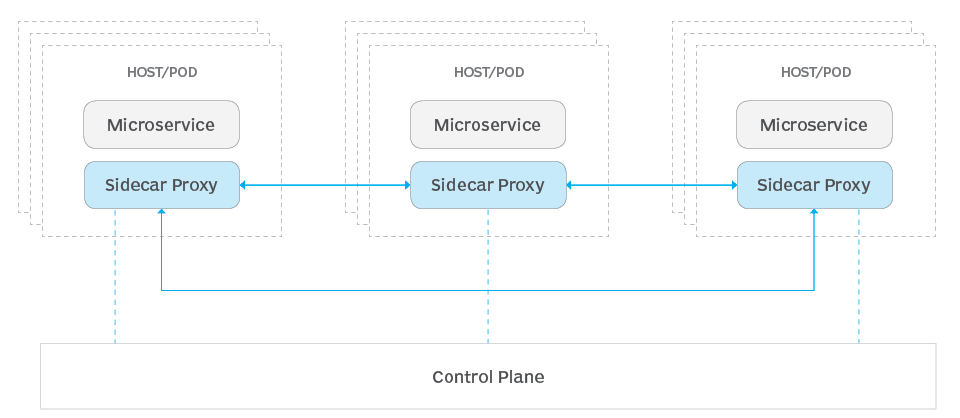
\includegraphics[width=16cm]{assets/literature-review/sidecar-proxy.png}
    \caption{Sidecar proxy design pattern \citep{Whatissi48:online}}
    \label{fig:sidecar-proxy}
    % https://cdn.ttgtmedia.com/rms/onlineimages/whatis-sidecar_proxy.png
\end{figure}

As this proxy sitting outside of the service, it is language-agnostic and intercepts all the inbound and outbound traffic at the application layer and relays them to the responsible parties. This is a very effective method to provide visibility into services without requiring additional work from developers. The main problem with this approach is that it adds a lot of network and CPU overhead to analyse requests with proxy \citep{Benchmar93:online}.

\begin{figure}[H]
    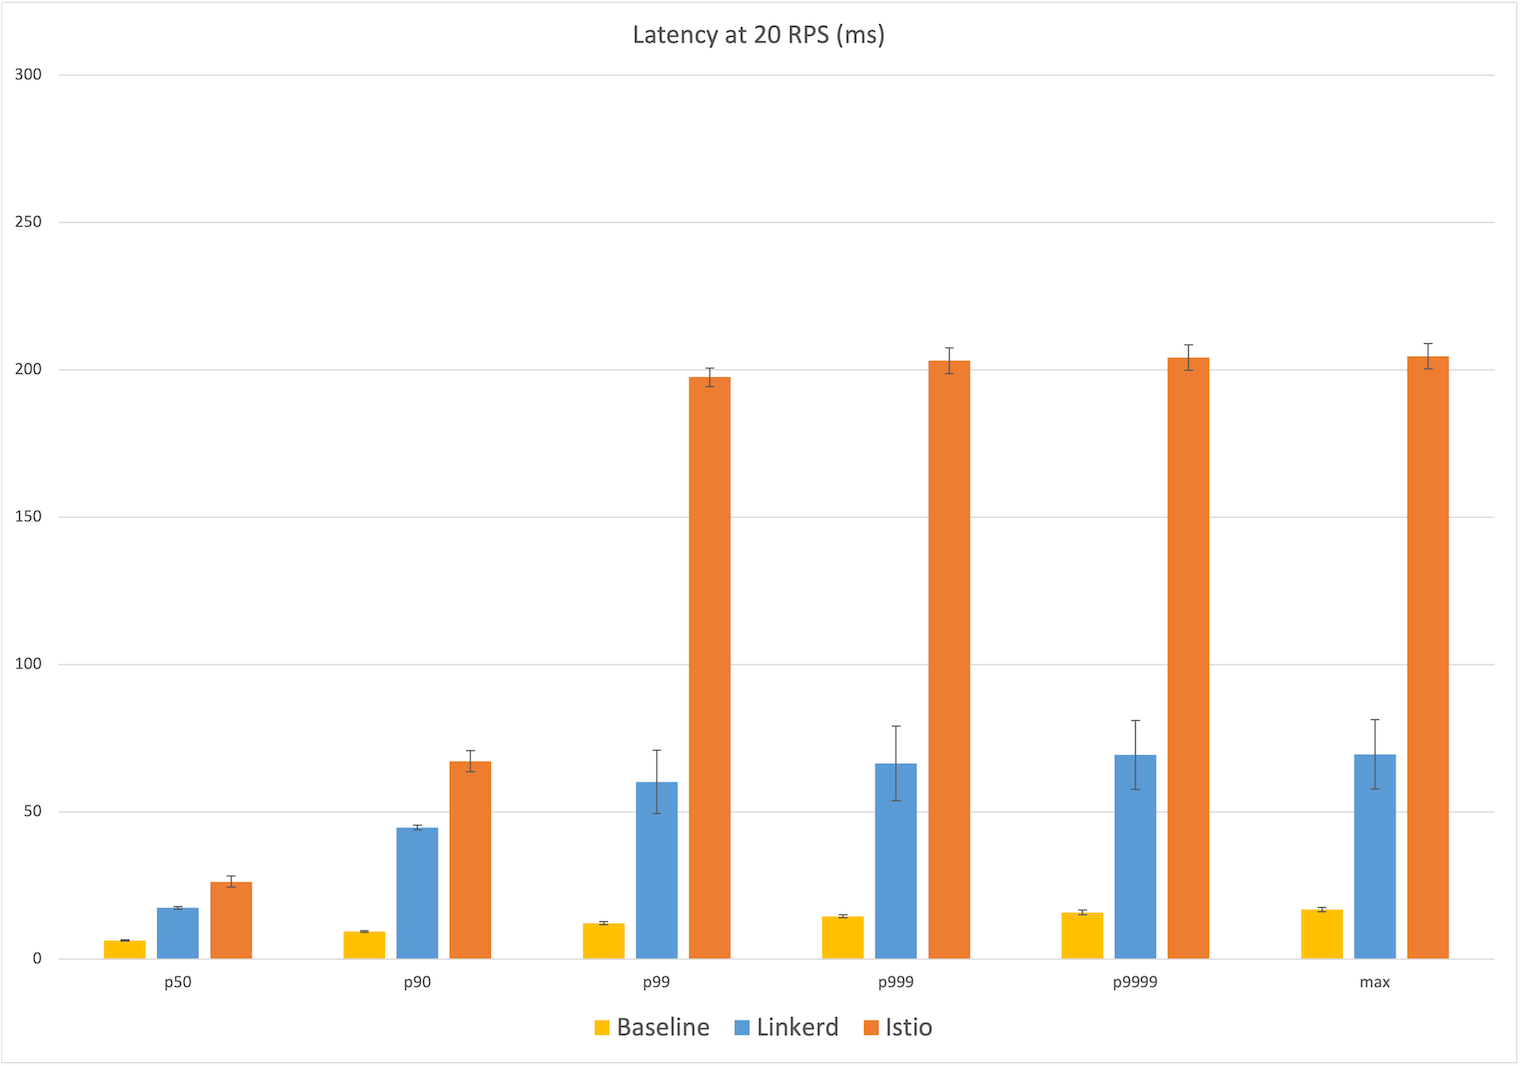
\includegraphics[width=11cm]{assets/literature-review/linkerd-benchmark.png}
    \caption{Service mesh benchmark \citep{Benchmar93:online}}
    \label{fig:linkerd-benchmark}
    % https://linkerd.io/images/benchmark/latency-20rps.png
\end{figure}

\subsubsection{Extended Berkeley Packet Filter (eBPF)}

\ac{ebpf} is a feature introduced to the Linux kernel in version 3.15 that allows deploying sandboxed programs to kernel space at runtime which could be used for application instrumentation from the kernel level \citep{LKMLIngo52:online}. \ac{ebpf} essentially created a way to run hooks on kernel events. For example kernel method "tcp\_v4\_syn\_recv\_sock" gets called every time a client wants to establish a TCP connection with the server. With \ac{ebpf}, users can deploy a lightweight hook that is called every time a new connection is made which will update the state on \ac{ebpf} map that could be read from user-space. 

\begin{figure}[H]
    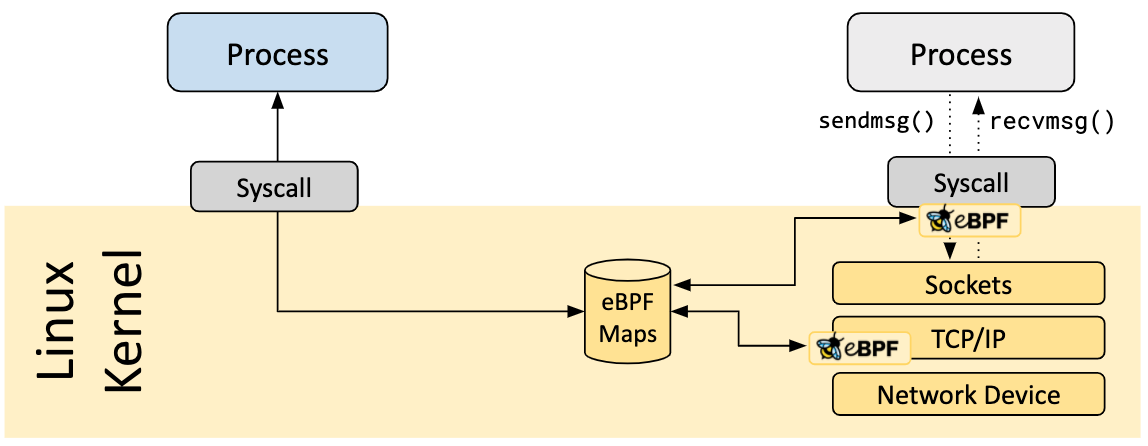
\includegraphics[width=11cm]{assets/literature-review/ebpf-architecture.png}
    \caption{eBPF architecture \citep{WhatiseB46:online}}
    \label{fig:ebpf-architecture}
    % https://ebpf.io/static/map\_architecture-e7909dc59d2b139b77f901fce04f60a1.png
\end{figure}

Using these data, the request rate of a given service can be calculated with minimum overhead and zero instrumentation on the application. The main drawback of this method is it is complicated to capture high-level data like HTTP status codes since those data only exist at the application level as it is.

\begin{longtable}{| p{23mm} | p{42mm} | p{42mm} | p{42mm} |}
\hline
    \textbf{Technique} &
    \textbf{Advantage} &
    \textbf{Disadvantage} &
    \textbf{Citations} \\ \hline

    Process Monitor &
    \vspace{-8mm}
    \begin{itemize}[leftmargin=0mm,noitemsep,nolistsep,label={}] 
        \item Virtually no overhead.
        \item Works out of the box.
        \vspace{-7mm}
    \end{itemize} &
    \vspace{-8mm}
    \begin{itemize}[leftmargin=0mm,noitemsep,nolistsep,label={}] 
        \item A very limited number of data points.
        \item     Not suited for a distributed system.
        \vspace{-7mm}
    \end{itemize} &
    \vspace{-8mm}
    \begin{itemize}[leftmargin=0mm,noitemsep,nolistsep,label={}] 
        \item \cite{chigurupati2017root}
        \item \cite{kumarage2018anomaly}
        \item \cite{kumarage2019generative}
        \vspace{-7mm}
    \end{itemize} \\ \hline

    Hypervisor Based Monitor &
    \vspace{-8mm}
    \begin{itemize}[leftmargin=0mm,noitemsep,nolistsep,label={}] 
        \item Most cloud providers provide a simple API to access these data.
        \vspace{-7mm}
    \end{itemize} &
    \vspace{-8mm}
    \begin{itemize}[leftmargin=0mm,noitemsep,nolistsep,label={}] 
        \item A limited number of data points
        \vspace{-7mm}
    \end{itemize} &
    \vspace{-8mm}
    \begin{itemize}[leftmargin=0mm,noitemsep,nolistsep,label={}] 
        \item \cite{du2018anomaly}
        \item \cite{geethika2019anomaly}
        \vspace{-7mm}
    \end{itemize} \\ \hline
    
    Service Mesh &
    \vspace{-8mm}
    \begin{itemize}[leftmargin=0mm,noitemsep,nolistsep,label={}] 
        \item In-depth monitoring,
        \item Request analysis, and modification at fly
        \item Framework Independent
        \vspace{-7mm}
    \end{itemize} &
    \vspace{-8mm}
    \begin{itemize}[leftmargin=0mm,noitemsep,nolistsep,label={}] 
        \item Performance Overhead
        \vspace{-7mm}
    \end{itemize} &
    \vspace{-8mm}
    \begin{itemize}[leftmargin=0mm,noitemsep,nolistsep,label={}] 
        \item \cite{samir2019dla}
        \item \cite{wu2020microrca}
        \vspace{-7mm}
    \end{itemize} \\ \hline
    
    Extended Berkeley Packet Filter &
    \vspace{-8mm}
    \begin{itemize}[leftmargin=0mm,noitemsep,nolistsep,label={}] 
        \item Very low overhead
        \item Works at the kernel level
        \item Able to scrape data related to the system
        \vspace{-7mm}
    \end{itemize} &
    \vspace{-8mm}
    \begin{itemize}[leftmargin=0mm,noitemsep,nolistsep,label={}] 
        \item Works only on Linux-based systems
        \item Difficult to develop and use
        \vspace{-7mm}
    \end{itemize} &
    \vspace{-8mm}
    \begin{itemize}[leftmargin=0mm,noitemsep,nolistsep,label={}] 
        \item None
        \vspace{-7mm}
    \end{itemize} \\ \hline

    \caption{Comparison of instrumentation methods (self-composed)}
\end{longtable}


\subsection{Detecting Anomalies}

\subsubsection{Supervised Learning}\label{sec:approch-supervised}
In general, The most popular way to detect anomalies is using supervised learning methods. Supervised learning methods can be implemented from finding outliers in sales patterns to fraud detection. \cite{du2018anomaly} As mentioned in the cloud computing domain, more than half of the methods are still based on supervised learning to detect anomalies. Among these Support Vector Machines (SVMs), Random Forest and Decision Trees were used the most. But one of the main downsides to using supervised learning in cloud computing is the lack of labeled anomalous data. Since most of the systems nowadays target at least 99\% of uptime finding labeled data is difficult. Even if there is a well-balanced dataset, the trained model won't be able to recognize unforeseen anomalies.

\subsubsection{Semi-Supervised Learning}

As mentioned in \ref{sec:approch-supervised}, one of the most challenging issues with anomaly detection is to find a data set with enough labelled abnormalities. One of the key factors contributing to the development of a well-generalised model is having a well-balanced data set \citep{batista2004study}. If the authors managed to find a sizable unbalanced data set, using clustering algorithms like K-nearest Neighbours (KNN) could yield better results. \cite{akcay2018ganomaly} managed to utilise an encoder-decoder-encoder architectural model to detect anomalies in image data and achieved remarkable results. 

\subsubsection{Unsupervised Learning}

When the target data set consists of a lot of unlabelled data and is difficult to label by hand, machine learning experts lean towards using unsupervised learning so the model can be its own teacher \citep{Unsuperv29:online}. \cite{silver2016mastering} managed to develop the first AI that was able to beat the best Go player in the world with a score of 4-1. This model learns to play the game of Go by looking at thousands of games played by humans and learning to approximate the optimal strategy to any given board position. One year later same authors released the updated version of the model which learn to play Go without any human interference and this model beated the previously published model 100-0 \citep{silver2017mastering}. This proves deep learning models could even surpass humans when it comes to finding patterns in very large distributions. 

\begin{longtable}{| p{23mm} | p{46mm} | p{42mm} | p{38mm} |}
\hline
    \textbf{Technique} &
    \textbf{Advantage} &
    \textbf{Disadvantage} &
    \textbf{Citations} \\ \hline
    
    Supervised Learning &
    \vspace{-8mm}
    \begin{itemize}[leftmargin=0mm,noitemsep,nolistsep,label={}] 
        \item Easy to develop and train.
        \item Models will converge better to the dataset.
        \item Easy to test the model performance.
        \item Ideal used for classification and regression problems.
        \vspace{-7mm}
    \end{itemize} &
    \vspace{-8mm}
    \begin{itemize}[leftmargin=0mm,noitemsep,nolistsep,label={}] 
            \item Require a labelled dataset.
            \item The models will not look at scenarios outside of the dataset. 
            \item The model will be biased if the labelled dataset was biased.
            \vspace{-7mm}
    \end{itemize} &
    \vspace{-8mm}
    \begin{itemize}[leftmargin=0mm,noitemsep,nolistsep,label={}] 
        \item \cite{du2018anomaly}
        \vspace{-7mm}
    \end{itemize} \\ \hline
    
    Semi-Supervised Learning &
    \vspace{-8mm}
    \begin{itemize}[leftmargin=0mm,noitemsep,nolistsep,label={}] 
        \item A blend of both Supervised and Unsupervised learning.
        \item Developers can force the model to learn some behaviors.
        \vspace{-7mm}
    \end{itemize} &
    \vspace{-8mm}
    \begin{itemize}[leftmargin=0mm,noitemsep,nolistsep,label={}] 
        \item Require a labeled dataset to train the initial steps.
        \item Model isn’t free to understand the problem from the ground up.
        \vspace{-7mm}
    \end{itemize} &
    \vspace{-8mm}
    \begin{itemize}[leftmargin=0mm,noitemsep,nolistsep,label={}] 
        \item \cite{akcay2018ganomaly}
        \vspace{-7mm}
    \end{itemize} \\ \hline
    
    Unsupervised Learning &
    \vspace{-8mm}
    \begin{itemize}[leftmargin=0mm,noitemsep,nolistsep,label={}] 
        \item Doesn’t require a labeled dataset.
        \item Excel at clustering extracting patterns from datasets.
        \vspace{-7mm}
    \end{itemize} &
    \vspace{-8mm}
    \begin{itemize}[leftmargin=0mm,noitemsep,nolistsep,label={}] 
        \item Developers have no control over the behaviour of the model.
        \vspace{-7mm}
    \end{itemize} &
    \vspace{-8mm}
    \begin{itemize}[leftmargin=0mm,noitemsep,nolistsep,label={}] 
        \item \cite{kumarage2018anomaly}
        \item \cite{zhang2019deep}
        \item \cite{kumarage2019generative}
        \item \cite{khoshnevisan2019rsm}
        \vspace{-7mm}
    \end{itemize} \\ \hline
    \caption{Comparison of anomaly detect methods in distributed systems (self-composed)}
\end{longtable}

\subsection{Root Cause Identification}

It's very difficult to use a standard learning algorithms like Multilayer Perceptrons (MLP) to predict faulty service because the number of microservices in distributed systems changes frequently. Even if the system were to retrain the model after every new deployment it will hesitate to predict newly added services as the root cause since it does not have any historical data about the service to make assumptions. Therefore, almost all published research uses the Key Performance Indicator (KPI) correlation or some variations of graph-based methods to predict the root cause of failures \citep{soldani2021anomaly}.

\begin{longtable}{| p{23mm} | p{42mm} | p{42mm} | p{42mm} |}
\hline
    \textbf{Technique} &
    \textbf{Advantage} &
    \textbf{Disadvantage} &
    \textbf{Citations} \\ \hline
    
    KPI correlation &
    \vspace{-8mm}
    \begin{itemize}[leftmargin=0mm,noitemsep,nolistsep,label={}] 
        \item Could find indirectly affected services.
        \item Easy to implement.
        \vspace{-7mm}
    \end{itemize} &
    \vspace{-8mm}
    \begin{itemize}[leftmargin=0mm,noitemsep,nolistsep,label={}] 
            \item The search space is large.
            \item Could result in a lot of false positives and noisy outputs. 
            \vspace{-7mm}
    \end{itemize} &
    \vspace{-8mm}
    \begin{itemize}[leftmargin=0mm,noitemsep,nolistsep,label={}] 
        \item \cite{nguyen2011pal}
        \item \cite{nguyen2013fchain}
        \item \cite{wang2020root}
        \vspace{-7mm}
    \end{itemize} \\ \hline
    
    Graph-based methods &
    \vspace{-8mm}
    \begin{itemize}[leftmargin=0mm,noitemsep,nolistsep,label={}] 
        \item Gives clear visual reasoning for the predications.
        \item  
        \vspace{-7mm}
    \end{itemize} &
    \vspace{-8mm}
    \begin{itemize}[leftmargin=0mm,noitemsep,nolistsep,label={}] 
        \item Miss out on indirectly affected components.
        \item Computing the causality graph could be expensive.
        \vspace{-7mm}
    \end{itemize} &
    \vspace{-8mm}
    \begin{itemize}[leftmargin=0mm,noitemsep,nolistsep,label={}] 
        \item \cite{samir2019dla}
        \item \cite{wu2020microrca}
        \item \cite{ma2020automap}
        \item \cite{meng2020localizing}
        \vspace{-7mm}
    \end{itemize} \\ \hline

    \caption{Comparison of root cause identification techniques (self-composed)}
\end{longtable}

\subsection{Evaluation}

Since this project consists of 3 components working together, finally all of these can be evaluated separately as the whole system.

To evaluate an instrumentation system, the author is hoping to use a static load generator like \href{https://github.com/MrSupiri/MicroSim}{MicroSim} to simulate a small microservices system and measure its performance of it by extracting CPU and Memory usage. Then gradually increase the complexity of the system and measure how the CPU and Memory usages change over the complexity of the system.

When it comes to data science, the data science component of this project is based on an unsupervised convolutional autoencoder. This model is trained on telemetry extracted from the system under normal behavior. The learning goal given in the model was to take the input and reconstruct it to the best of its ability. Due to the architecture autoencoders doing, it will force the model to learn the relationship between each metric and how it corresponds with each other. Since the model's output never be a perfect recreation of the input traditional metrics like Precision, Recall, and F1 Score can not be used. Instead, the only metric that can be tracked during the training and testing is the reconstruction loss \citep{ghasedi2017deep}. The final output presented to the user end of this research will be the servie's predicted health. This value will be derived by getting the difference between the highest and lowest possible value for reconstruction loss and calculating which percentile it belongs to.